% Template for BiDS'19 papers; to be used with:
%          spconf.sty  - LaTeX style file, and
% --------------------------------------------------------------------------
\documentclass{article}
\usepackage{spconf,amsmath,epsfig}

\providecommand{\doi}[1]{doi: {\footnotesize \href{http://dx.doi.org/#1}{\path{#1}}}}

\usepackage[pdftex=true,breaklinks=true,hidelinks=true,colorlinks=true,citecolor=blue]{hyperref}

\usepackage[square,numbers]{natbib}
\renewcommand{\bibsection}{\section*{\normalsize\hspace*{\fill}REFERENCES\hspace*{\fill}}}


% Example definitions.
% --------------------
\def\x{{\mathbf x}}
\def\L{{\cal L}}

% Title.
% ------
\title{THE PANGEO BIG DATA ECOSYSTEM AND ITS USE AT CNES}
%
% Single address.
% ---------------
\name{Guillaume Eynard-Bontemps, Joseph Hamman, Ryan Abernathey, Matthew Rocklin, Aurélien Ponte}%\thanks{Thanks to XYZ agency for funding.}}
\address{CNES, NCAR, Columbia, Anaconda, Ifremer}
%
% For example:
% ------------
%\address{School\\
%	Department\\
%	Address}
%
% Two addresses (uncomment and modify for two-address case).
% ----------------------------------------------------------
%\twoauthors
%  {A. Author-one, B. Author-two\sthanks{Thanks to XYZ agency for funding.}}
%	{School A-B\\
%	Department A-B\\
%	Address A-B}
%  {C. Author-three, D. Author-four\sthanks{The fourth author performed the work
%	while at ...}}
%	{School C-D\\
%	Department C-D\\
%	Address C-D}
%
\begin{document}
%\ninept
%
\maketitle
%
\begin{abstract}
Pangeo\cite{b1} is a community driven effort for open-source big-data intially focused on the Earth System Sciences. It represents at the same time a collaboration of people and a platform composed of open source scientific python packages like Jupyter, Dask and Xarray. One of its goal is to improve scalability of these tools to handle petabyte-scale datasets on HPC or public cloud infrastructure.
In this paper, we will first describe Pangeo: its motivation, community, the underlying technology stack and associated deployments, different applications and the on going work. On a second part, we will present its use in CNES: HPC deployment, some simple and more complicated use cases, and what we are planning to do.
\end{abstract}
%
\begin{keywords}
Pangeo, Dask, Jupyter, HPC, Cloud, Big Data, Analysis
\end{keywords}
%
\section{Pangeo}
\label{sec:pangeo}

\subsection{Motivations, mission and goals}
\label{ssec:motivations}

There are several building crises facing the geoscience community:

\begin{itemize}
\item Big Data: datasets are growing too rapidly and legacy software tools for scientific analysis can’t handle them. This is a major obstacle to scientific progress.
\item Technology Gap: a growing gap between the technological sophistication of industry solutions (high) and scientific software (low).
\item Reproducibility: a fragmentation of software tools and environments renders most geoscience research effectively unreproducible and prone to failure.
\end{itemize}

Pangeo aims to address these challenges through a unified, collaborative effort.

Our mission is to cultivate an ecosystem in which the next generation of open-source analysis tools for ocean, atmosphere and climate science can be developed, distributed, and sustained. These tools must be scalable in order to meet the current and future challenges of big data, and these solutions should leverage the existing expertise outside of the geoscience community.

To accomplish this mission, we have identified three specific goals.
\begin{itemize}
\item Foster collaboration around the open source scientific python ecosystem for ocean / atmosphere / land / climate science.
\item Support the development with domain-specific geoscience packages.
\item Improve scalability of these tools to handle petabyte-scale datasets on HPC and cloud platforms.
\end{itemize}

\subsection{Community}
\label{ssec:community}

One crutial attribute of Pangeo is to be community driven. The goal is of course to have the most wider and open comunity as possible. All the effort are made in the open on github, any one can join or get involved in the community. 

The community is already quite diverse, from academic research, going through government agency up to open source developers. A lot of different nationalities are represented too: from USA of course, but also UK, France or Australia to name a few.

\subsection{Technology stack}
\label{ssec:techstack}

Jupyter/Dask/Xarray scheme \ref{pangeo_stack} and explanation.

Present all three, the cloud and HPC also.

\begin{figure}
  \centering
  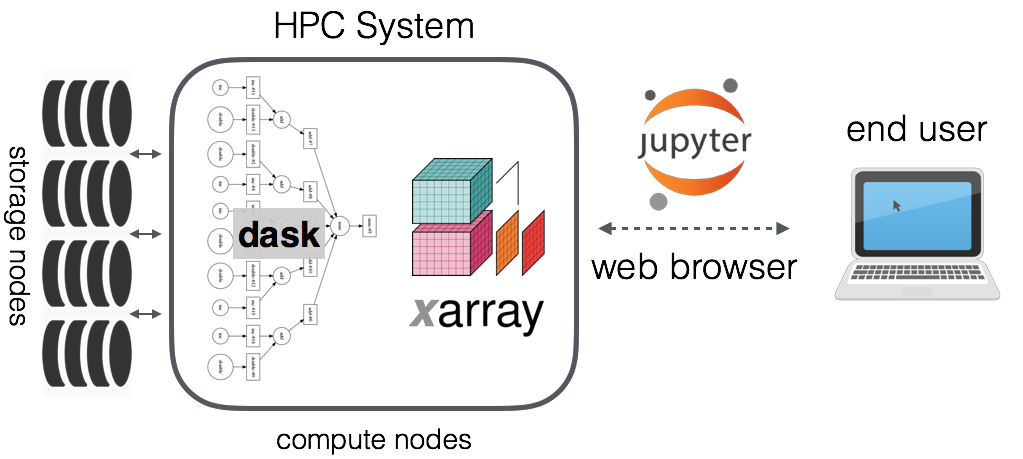
\includegraphics[width=\columnwidth]{pangeo_stack.png}
  \caption{\label{pangeo_stack} Pangeo platform main components.}
\end{figure}

\subsection{Applications}
\label{ssec:applications}

Go through one Pangeo example and also the last blog post from Scott Henderson.

\subsection{On going work}
\label{ssec:ongowork}

Binder, Community governance, subdomains and Continuous deployment, Cluster Manager rationalization...

\section{CNES deployment and use cases}
\label{sec:cnes}

\subsection{Context and HPC System}
\label{ssec:context}

CNES various science, heavy simulations through launchers or flight dynamics, but majority of data processing : remote sensing, astronomy, climate.

Main processing platform is our cluster HAL: modestly sized High Performance Computer: 8000 cores, 6PB storage. PBS Pro.

\subsection{From embarrassingly parallel to more complex workflow with Dask}
\label{ssec:usecase1}

Embarrassingly parallel simulation

Before: complex and unreadable batch scripts, launching PBS arrays, writting millions of small results on shared storage.

With Dask: elegant python code, scaling easily, in memory data exchange...

Add some post processing

Add some CSV file generation, build of a dask dataframe, reduction of results, launch of a new simulation...

\subsection{Simulating remote sensing data through dask array}
\label{ssec:usecase2}

Generating a lot of Dask array that needs to be sum.
Memory problem, rechunking...

\ref{fig_example} and Fig. \ref{fig:res}.

% Below is an example of how to insert images. Delete the ``\vspace'' line,
% uncomment the preceding line ``\centerline...'' and replace ``imageX.ps''
% with a suitable PostScript file name.
% -------------------------------------------------------------------------
\begin{figure}
  \centering
  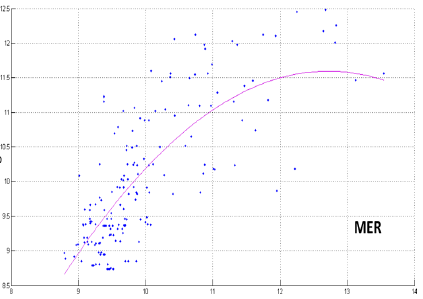
\includegraphics[width=\columnwidth]{figure.png}
  \caption{\label{fig_example} Result 1.}
\end{figure}

\begin{figure}

\begin{minipage}[b]{.48\linewidth}
  \centering
  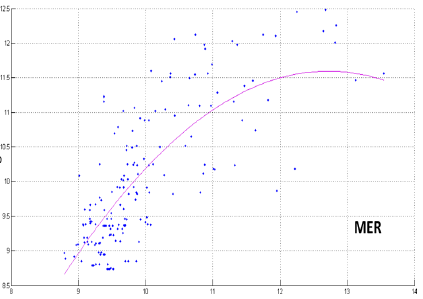
\includegraphics[width=\columnwidth]{figure.png}
% \centerline{\epsfig{figure=image3.ps,width=4.0cm}}
 % \vspace{1.5cm}
  \centerline{(a) Results 2}\medskip
\end{minipage}
\hfill
\begin{minipage}[b]{0.48\linewidth}
  \centering
  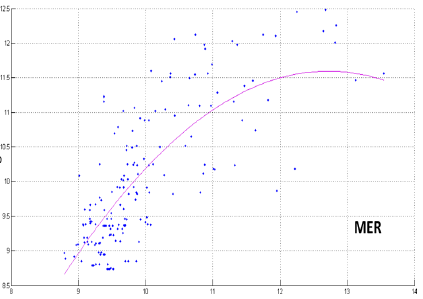
\includegraphics[width=\columnwidth]{figure.png}
% \centerline{\epsfig{figure=image4.ps,width=4.0cm}}
  %\vspace{1.5cm}
  \centerline{(b) Result 3}\medskip
\end{minipage}
%
\caption{Example of placing two figures with experimental results.}
\label{fig:res}
%
\end{figure}


% To start a new column (but not a new page) and help balance the last-page
% column length use \vfill\pagebreak.
% -------------------------------------------------------------------------
\vfill
\pagebreak


% References should be produced using the bibtex program from suitable
% BiBTeX files 
% -------------------------------------------------------------------------

\bibliographystyle{plainnat}
\bibliography{myBibFile}

\small

\begin{thebibliography}{00}
\bibitem{b1} Abernathey, Ryan; paul, kevin; hamman, joe; rocklin, matthew; lepore, chiara; tippett, michael; et al. (2017): Pangeo NSF Earthcube Proposal. figshare. \href{https://figshare.com/articles/Pangeo_NSF_Earthcube_Proposal/5361094}{Figshare paper}. 
\end{thebibliography}

\end{document}
